% =============================================================================
% Section 7 — Variant Landscapes from Live Databases
% =============================================================================
\section{Variant Landscapes: What the Databases Actually Say}\label{sec:variants}

\begin{objectives}
\begin{itemize}[leftmargin=*,itemsep=1pt,topsep=1pt]
  \item Retrieve gene, protein and variant records from Ensembl, UniProt, InterPro and ClinVar.
  \item Locate a variant within a protein domain and verify the claim rather than assert it.
  \item Read ClinVar base rates correctly, including why its categories do not partition.
  \item Recognise the reference-assembly and overlap pitfalls that corrupt variant arguments.
\end{itemize}
\end{objectives}

\subsection{Why retrieve rather than quote}

Every identifier in this book is fetched from a public endpoint and cached with
its URL and a UTC timestamp, by
\file{scripts/textbook/retrieve_genomic_data.py}. There are two reasons, and the
second is the important one.

The obvious reason is reproducibility. The deeper reason is that \emph{retrieval
can fail a claim}. When the script is run, it checks its own output: that every
gene record is on GRCh38, that every domain lies inside its protein, and that
residue $286$ falls within the retrieved boundaries of \texttt{IPR006133}. If any
check fails it refuses to write the cache. An assertion in prose cannot do that.

\subsection{What the records say}

\begin{table}[htbp]
\centering
\caption{Gene records retrieved from Ensembl REST, GRCh38. The replicative
polymerases of Sections~\ref{sec:proofreading}--\ref{sec:refutation} and the
mismatch-repair genes of Section~\ref{sec:mmr}.}
\label{tab:genes}
\begin{tabularx}{\linewidth}{@{}l l r r X@{}}
\toprule
\textbf{Gene} & \textbf{Ensembl ID} & \textbf{Chr} & \textbf{Span (bp)} & \textbf{Role here} \\
\midrule
\texttt{POLE}  & \texttt{ENSG00000177084} & 12 & $63\,624$  & leading-strand polymerase; the variant \\
\texttt{POLD1} & \texttt{ENSG00000062822} & 19 & $33\,815$  & lagging-strand polymerase; comparison \\
\texttt{MSH6}  & \texttt{ENSG00000116062} & 2  & $114\,580$ & MMR recognition; the $\textsf{msh6}\Delta$ of §\ref{sec:mmr} \\
\texttt{MSH2}  & \texttt{ENSG00000095002} & 2  & $260\,080$ & MMR recognition partner \\
\texttt{MLH1}  & \texttt{ENSG00000076242} & 3  & $58\,672$  & MMR effector \\
\bottomrule
\end{tabularx}
\end{table}

The protein picture is where the argument of Section~\ref{sec:refutation} is
anchored. \texttt{POLE} (UniProt \texttt{Q07864}) is $2286$ residues. InterPro
places five domains on it; the one that matters is \texttt{IPR006133}, the
family-B DNA polymerase exonuclease domain, at residues $220$--$426$.

\begin{figure}[htbp]
  \centering
  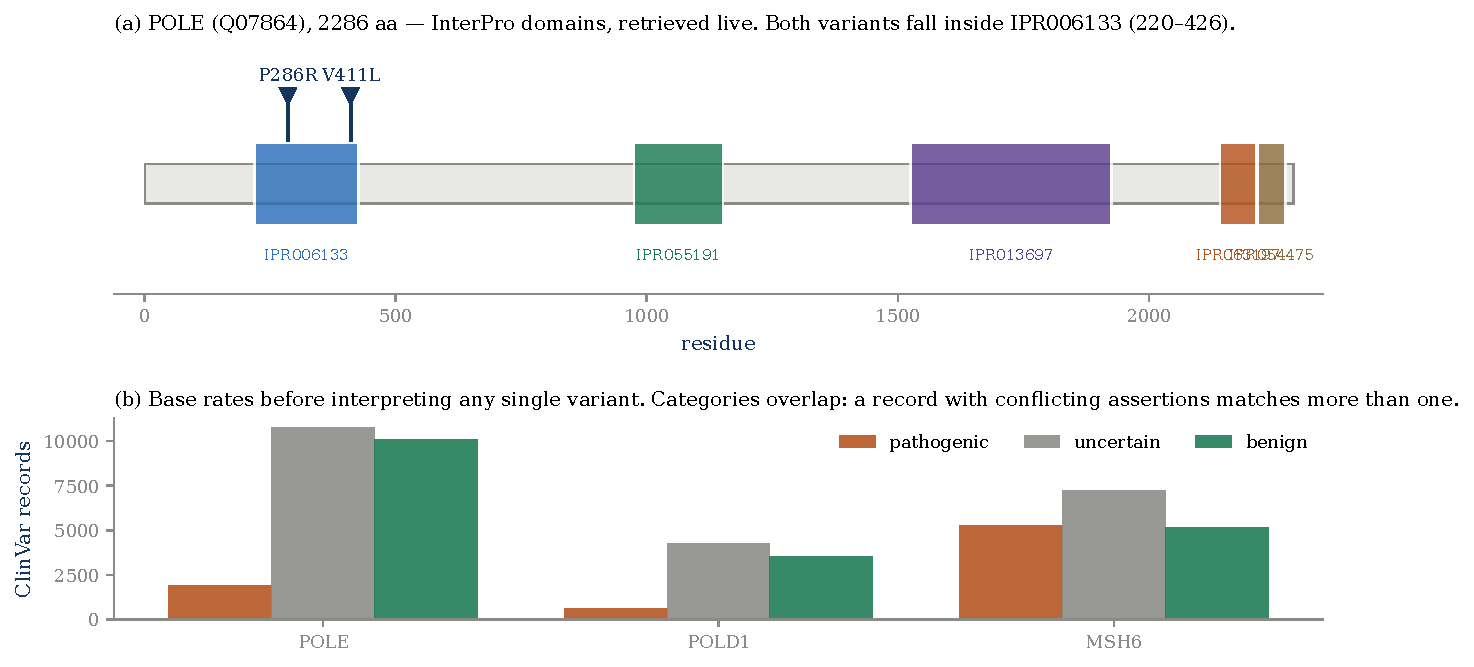
\includegraphics[width=\textwidth]{fig07_variant_landscape.pdf}
  \caption{(a) \texttt{POLE} domain architecture from InterPro, drawn to scale,
  with the two variants discussed in this book marked. Both \texttt{P286R} and
  the neutral control \texttt{V411L} fall inside the exonuclease domain --- which
  is itself instructive: being in the proofreading domain does not make a variant
  a mutator, as Section~\ref{sec:refutation}'s control shows. (b) ClinVar record
  counts. Note that the categories overlap.}
  \label{fig:landscape}
\end{figure}

\subsection{Reading ClinVar without being misled}

Figure~\ref{fig:landscape}(b) reports, for \texttt{POLE}: $1891$ records matching
``pathogenic'', $10\,065$ matching ``benign'', $10\,737$ matching ``uncertain
significance'', against $11\,341$ records in total.

Those numbers sum to $22\,693$, twice the total. This is not an error in the
retrieval, and the fact is worth dwelling on because it trips people up
constantly: \textbf{ClinVar's clinical-significance categories do not partition
the records}. A variant with conflicting submissions matches more than one
filter. Any argument of the form ``$x\%$ of variants in this gene are pathogenic,
computed as pathogenic over total'' is therefore wrong.

\begin{remark}[The base-rate discipline]
Before interpreting any individual variant, look at the gene's base rates.
\texttt{POLE} has $1891$ pathogenic-matching records against $10\,737$ of
uncertain significance. The modal outcome of finding a novel \texttt{POLE}
missense variant in a patient is \emph{not} a diagnosis; it is a VUS. A method
that confidently classifies such variants should be viewed against that base
rate, not against its own accuracy on curated examples.
\end{remark}

\begin{worked}[7.1: a variant in the right domain that does nothing]
\textbf{Problem.} \texttt{V411L} lies at residue $411$, inside \texttt{IPR006133}
($220$--$426$), the same domain as \texttt{P286R}. Yet Section~\ref{sec:refutation}
used it as a \emph{negative} control: it does not break the PSR$_2$ ceiling. Is
this a contradiction?

\textbf{Solution.} No, and the apparent tension is the point of the exercise.
Domain membership is a statement about \emph{where} a residue sits in a sequence
annotation; mutator phenotype is a statement about \emph{what} the substituted
protein does. Localisation is evidence of opportunity, not of effect.

Concretely: the exonuclease domain contains catalytic residues, metal-coordinating
residues, structural residues and surface residues. A substitution at a surface
position inside the domain may leave catalysis untouched. Inferring function from
domain membership is the same category error that Section~\ref{sec:proof-and-cell}
warned about --- treating a modelling claim (``in the domain, therefore disrupts
the domain'') as though it were established.
\end{worked}

\begin{exercise}
Using Table~\ref{tab:genes}, compute the genomic span of \texttt{MSH2} in
kilobases and compare it with \texttt{POLE}. Does a larger gene imply more
ClinVar records? Check against Figure~\ref{fig:landscape}(b) and comment.
\end{exercise}

\begin{exercise}
A colleague computes ``the pathogenic fraction of \texttt{MSH6}'' as
$5289/10\,849 = 48.8\%$ and concludes that \texttt{MSH6} variants are more often
pathogenic than not. Identify two independent errors in this reasoning.
\end{exercise}

\begin{exercise}
The retrieval script asserts that every gene record carries
\texttt{assembly == "GRCh38"}. Explain what could go wrong in a variant analysis
if records from GRCh37 and GRCh38 were mixed, and why a coordinate alone is not
a variant identifier.
\end{exercise}

\begin{exercise}[(harder)]
Section~\ref{sec:refutation} relies on the yeast allele \texttt{pol2-P301R} being
the analogue of human \texttt{P286R}. Using the UniProt and InterPro records,
describe the evidence you would need to justify that correspondence, and state
what the argument assumes that the databases do not supply.
\end{exercise}

\begin{ledger}
\textbf{Measured:} all records in Table~\ref{tab:genes} and
Figure~\ref{fig:landscape}, retrieved live from Ensembl REST, UniProt, InterPro
and NCBI E-utilities; URLs and timestamps in
\file{textbook/data/genomic_records.json}. \\
\textbf{Assumed:} that the canonical/MANE transcript is the appropriate
coordinate frame, and that InterPro domain boundaries are an adequate proxy for
functional boundaries. The second is weaker than it looks --- see
Worked Example~7.1. \\
\textbf{Proved:} nothing formalised. The retrieval script's internal consistency
checks are assertions over fetched data, not theorems: they can fail at runtime,
which is their purpose. \\
\textbf{Open:} the yeast-to-human correspondence of Exercise~7.4 is assumed
throughout this book and is nowhere established in it.
\end{ledger}
